\def\na{94\xspace}
\def\ni{40\xspace}
The search yielded 1384 publications,
of which \na studies were included
(Figure~\ref{fig:prisma}).
360 studies used dynamical HIV transmission models applied to SSA, of which
255 were compartmental models. 
\na compartmental modeling studies simulated ART scale-up (Database~A), of which
\ni reported infections averted or incidence reduction
due to population-wide ART scale-up without additional combination interventions,
as compared to a base case reflecting status quo (Database~B).
Appendix~\ref{aa:search:database} lists the included papers, and
Appendix~\ref{a:results} provides additional results.
\begin{figure}[h]
  \centering
  \newcommand{\nprisma}[2]{\textbf{#2} (N~{=}~#1)}%
\newcommand{\nprismasub}[2]{\parbox{4ex}{\hfill#1}: #2\\}%
\begin{tikzpicture}[xscale=5.5,yscale=1.8]
  \scriptsize
  % boxes
  \node[prisma](a0) at (0, 0.0) {\nprisma{2134}{Database search hits\\}};
  \node[prisma](a1) at (1, 0.0) {\nprisma {767}{Duplicates removed automatically\\}};
  \node[prisma](b0) at (0,-1.0) {\nprisma{1367}{Abstracts screened\\}};
  \node[prisma](b1) at (1,-1.0) {\nprisma {595}{Irrelevant\\}};
  \node[prisma](c0) at (0,-2.0) {\nprisma {772}{Full texts assessed\\}};
  \node[prisma](c1) at (1,-2.0) {\nprisma {424}{Excluded}\\\raggedright
    \nprismasub{  4}{Duplicate}
    \nprismasub{115}{Publication type}
    \nprismasub{118}{No transmission modelling}
    \nprismasub{136}{Not dynamical model}
    \nprismasub{ 12}{Not SSA}
    \nprismasub{ 25}{Not HIV}
    \nprismasub{ 17}{Model comparison}};
  \node[prisma](d0) at (0,-3.7) {\nprisma{360}{Dynamical HIV transmission model\\}};
  \node[prisma](d1) at (1,-3.7) {\nprisma{266}{Excluded}\\\raggedright
    \nprismasub{105}{Individual-based model}
    \nprismasub{161}{No ART scale-up scenario}};
  \node[prisma](e0) at (0,-4.7) {\nprisma{94}{Any ART scale-up scenario\\}\\\textit{Dataset~A}};
  \node[prisma](e1) at (1,-4.7) {\nprisma{54}{Excluded}\\\raggedright
    \nprismasub{23}{Only combination interventions}
    \nprismasub{14}{Reported other measures}
    \nprismasub{ 8}{No status quo base case scenario}
    \nprismasub{ 4}{Only ART targeted to risk groups}
    \nprismasub{ 1}{Repeated modelling analysis}};
  \node[prisma](f0) at (0,-5.7) {\nprisma{40}{Infections averted / incidence reduction due to ART scale-up for all\\}\\\textit{Dataset~B}};
  % arroes
  \draw[arrow] (a0) -- (a1);
  \draw[arrow] (a0) -- (b0);
  \draw[arrow] (b0) -- (b1);
  \draw[arrow] (b0) -- (c0);
  \draw[arrow] (c0.east) -- (c1.west|-c0.east);
  \draw[arrow] (c0) -- node[right]{$+$12 Cited Studies} (d0);
  \draw[arrow] (d0.east) -- (d1.west|-d0.east);
  \draw[arrow] (d0) -- (e0);
  \draw[arrow] (e0.east) -- (e1.west|-e0.east);
  \draw[arrow] (e0) -- (f0);
\end{tikzpicture}
\vskip 1ex
  \caption{PRISMA flowchart of study identification}
  \label{fig:prisma}
\end{figure}
% ==============================================================================
\subsection{Epidemic Context}
\label{ss:res:context}
Table~\ref{tab:summary} summarizes the key features of contexts within SSA
where the prevention impacts of ART have been modelled.
Most (\x{geo/n.any.nat}) of the \na studies modelled HIV transmission at the national level,
including \x{geo/n.nat} single-country and \x{geo/n.nat.multi} multi-country analyses.
Studies also explored
regional (\x{geo/n.any.sub.ssa}),
sub-national (\x{geo/n.any.sub.nat}), and
city-level (\x{geo/n.any.city}) epidemic scales.
South Africa was the most common country simulated (\x{co/n.South-Africa} studies),
but was not disproportionately represented among SSA countries:
the number of studies per million PLHIV as of 2019 in South Africa (\x{co/mph.South-Africa})
was similar to the SSA median (\x{co/mph.med}).
Figure~\ref{fig:map} illustrates the number of studies by country.
East Africa was the most represented SSA region being simulated in \x{co/n.re.east} studies,
followed by Southern (\x{co/n.re.south}), Central (\x{co/n.re.central}), and West Africa (\x{co/n.re.west}).
\begin{table}
  \centering
  \caption{Summary of epidemic contexts within Sub-Saharan Africa where
    the prevention impacts of ART have been modelled}
  \label{tab:summary}
  \footnotesize\singlespacing
\begin{tabular}{llr}
	\toprule
	\multicolumn{2}{l}{Study Characteristic} & Studies               \\
	\midrule
	Geographic scale & Regional              & \x{geo/n.any.sub.ssa} \\
	                 & National              & \x{geo/n.any.nat}     \\
	                 & Sub-national          & \x{geo/n.any.sub.nat} \\
	                 & City                  & \x{geo/n.any.city}    \\
	\midrule
	Modelled         & South Africa          & \x{co/n.South-Africa} \\
	countries\tn{a}  & Kenya                 & \x{co/n.Kenya}        \\
	                 & Zambia                & \x{co/n.Zambia}       \\
	                 & Other                 & \x{co/n.Other}        \\
	\midrule
	HIV prevalence   & Low ($<$1\%)          & \x{t0/n.prev.Low}     \\
	                 & Mid (1-10\%)          & \x{t0/n.prev.Mid}     \\
	                 & High ($>$10\%)        & \x{t0/n.prev.High}    \\
	                 & Unclear/Varies        & \x{t0/n.prev.NA}      \\
	\midrule
	Incidence trend  & Decreasing            & \x{t0/n.phase.decr}   \\
	at scenario      & Dec-to-stable         & \x{t0/n.phase.dts}    \\
	divergence       & Stable                & \x{t0/n.phase.stab}   \\
	                 & Inc-to-stable         & \x{t0/n.phase.its}    \\
	                 & Increasing            & \x{t0/n.phase.incr}   \\
	                 & Unclear/Varies        & \x{t0/n.phase.NA}     \\
	\midrule
	Key populations  & FSW\tn{b}             & \x{kp/n.FSW}          \\
	included         & Clients\tn{c}         & \x{kp/n.Cli}          \\
	                 & MSM                   & \x{kp/n.MSM}          \\
	                 & PWID                  & \x{kp/n.PWID}         \\
%	                 & AGYW                  & TODO                  \\
	\bottomrule
\end{tabular}
\floatfoot{
  Total studies: \na.
  FSW: female sex workers;
  Clients: clients of sex workers;
  MSM: men who have sex with men;
  PWID: people who inject drugs;
%  AGYW: adolescent girls and young women;
%  MP: mobile populations.
  \tnt[a]{Does not sum to \na as some studies modelled multiple countries}.
  \tnt[b]{FSW as defined by three epidemiological criteria in Appendix~\ref{aaa:defs:kp};
    \x{kp/n.FSW.n.crit.3} met all three FSW criteria while
    \x{kp/n.FSW.n.crit.NA} were described as FSW but the criteria could not be evaluated;
    another \x{kp/n.FSW.n.crit.fail} were described as FSW but did not meet the criteria.}
  \tnt[c]{Likewise for clients, the counts were:
    \x{kp/n.Cli.n.crit.1},~\x{kp/n.Cli.n.crit.NA},~and~\x{kp/n.Cli.n.crit.fail}, respectively.}
}

\end{table}
\begin{figure}[h]
  \centering
  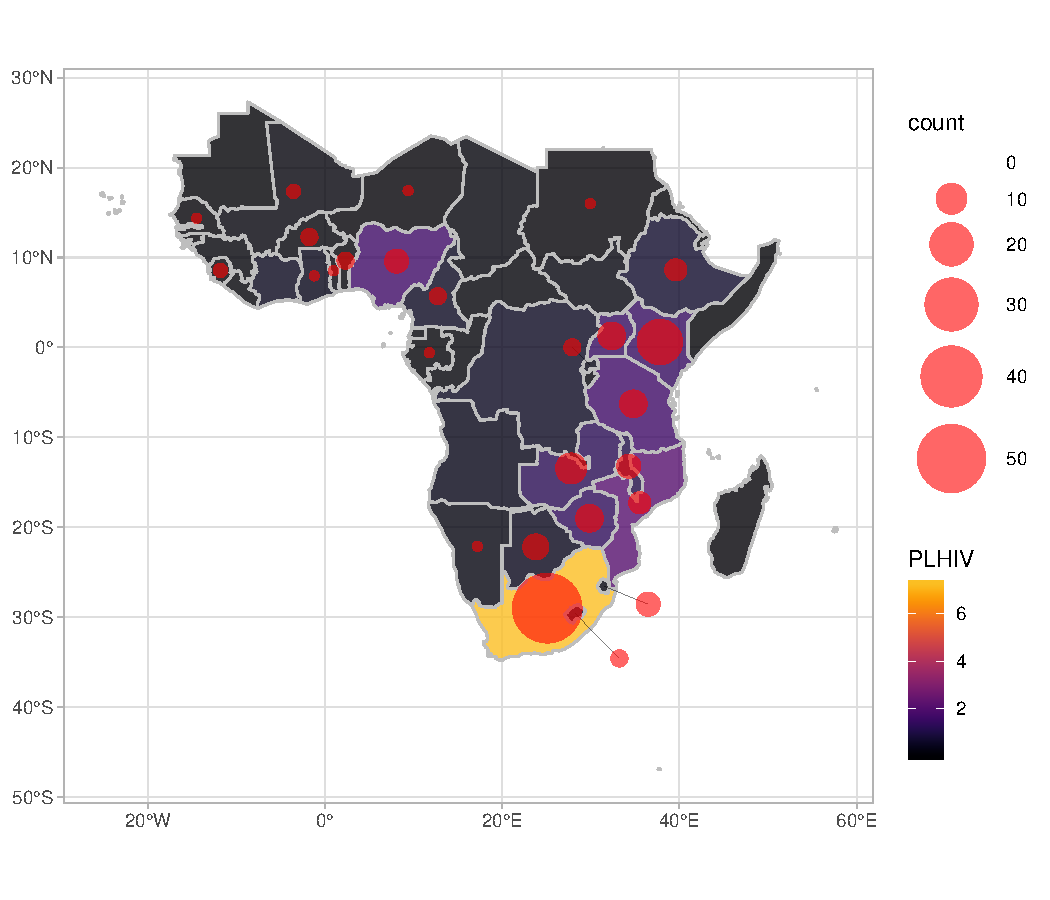
\includegraphics[width=0.8\linewidth]{map-n-vs-plhiv}
  \caption{Map showing number of studies (of \na total)
    applying HIV transmission modelling in each country vs
    the number of people living with HIV (PLHIV, millions)}
  \label{fig:map}
\end{figure}
\par
ART prevention impacts were most often modelled in
high-prevalence epidemics (${>10\%}$ HIV prevalence, \x{t0/n.prev.High} studies) and
medium-prevalence epidemics (${1-10\%}$, \x{t0/n.prev.Mid} studies).
No studies reported overall HIV prevalence of ${<1\%}$ at time of ART scale-up,
although for \x{t0/n.prev.NA} studies, HIV prevalence was either
not reported or varied across independently simulated contexts/scenarios.
The \xdmdef year of scenario ART scale-up was \xdm{t0/t0}; at which time
HIV prevalence (\%) was \xdm{t0/prev}; and
incidence (per 1000 PY) was \xdm{t0/inc}.
Most contexts reporting incidence trends had decreasing or stable incidence
(45 of 48 reporting). % MAN \x{t0/n.phase.*}
\subsubsection{Key Populations}
\label{sss:res:kp}
% JK: TODO
FSW were defined based on a combination of  %SM: rephrase sentence for clarity 
being described as FSW by the study and three epidemiological criteria.
Among \x{kp/n.FSW.named} studies describing FSW activity groups:
all three criteria were satisfied in \x{kp/n.FSW.n.crit.3} studies;  %SM: don't follow...
the criteria were either satisfied or indeterminate and assumed to be satisfied
in another \x{kp/n.FSW.n.crit.NA};
and were not satisfied in \x{kp/n.FSW.n.crit.fail}.
Among studies that did not describe FSW activity groups,
none satisfied all three criteria.  %SM: i don't remeber reading about criteria in the methods about this - but maybe I missed it?
\par
Among \x{kp/n.Cli.named} studies describing clients of FSW:
\x{kp/n.Cli.n.crit.1} met the epidemiological criteria;
\x{kp/n.Cli.n.crit.NA} were indeterminate and assumed to meet the criteria; and
\x{kp/n.Cli.n.crit.fail} did not meet the criteria.
Another \x{kp/n.Cli.p} described clients as a proportion of another male risk group.
\par
Activity groups described as representing
men who have sex with men (MSM) were noted in \x{kp/n.MSM} studies;
people who inject drugs (PWID) in \x{kp/n.PWID}.
% No epidemiological criteria were employed to formalize these definitions.
% \par
% adolescent girls and young women (AGYW) in [TODO].
% mobile populations [TODO].
% ==============================================================================
\subsection{Heterogeneity Factors}
\label{ss:res:factors}
% ------------------------------------------------------------------------------
\subsubsection{Biological Effects}
\label{sss:res:bio}
The \xdmdef number of states used to represent HIV disease
(ignoring treatment-related stratifications) was \xdm{hiv/hiv.n},
and \x{hiv/n.hiv.cts} studies represented HIV along a continuous dimension
using a partial differential equations model.
Most HIV states were defined by CD4 count % JK: TODO count?
to reflect clinical progression and/or historical ART eligibility,
often with additional states to represent acute infection and/or development of AIDS.
% \x{hiv/n.hiv.def.VL} minority of models considered both CD4 count and viral load as separate dimensions.
States of increased infectiousness associated with acute infection and late stage disease
were simulated in \x{hiv/n.hiv.acute} and \x{hiv/n.hiv.late} studies, respectively.
% All \na studies included increased mortality associated with HIV infection.
\par
The relative risk of HIV transmission on ART was \xdm{art/rbeta},
representing an average ``on-treatment'' state in \x{art/n.rbeta.x.T} studies,
vs a ``virally suppressed'' state specifically in \x{art/n.rbeta.x.V} studies.
% \x{distr/n.rbeta.x.NA} unclear = 1
% Male circumcision was simulated in \x{act/n.mc} studies.
% Coinfection with other STI and TB was simulated \x{hiv/coinf.sti} and \x{hiv/coinf.tb}, respectively.
Treatment failure due to drug resistance was simulated in \x{art/n.art.fail.any} studies, including:
\x{art/n.art.x.fail} using a separate ``treatment failure'' compartment;
\x{art/n.art.x.fail} using a transition back into a generic ``off-treatment'' HIV state; and another
\x{art/n.art.r.frop} in which a similar transition  was not clearly identified as treatment failure vs dropout.
Transmissible drug resistance was simulated in \x{art/n.tdr} studies.
% ------------------------------------------------------------------------------
\subsubsection{Behavioural Effects} %SM: try to use more active voice
\label{sss:res:beh}
Reduced sexual activity during late-stage HIV symptoms was simulated in \x{hiv/n.hiv.morb.any} studies,
including at least one state with:
complete cessastion of sexual activity (\x{hiv/n.hiv.morb.inact});
reduced rate or number of partnerships (\x{hiv/n.hiv.morb.np}); and/or
reduced rate or number of sex acts per partnership (\x{hiv/n.hiv.morb.vol}).
\par
Separate health states representing diagnosed HIV but not yet on treatment
and on treatment but not yet virally suppressed were simulated in
\x{art/n.art.x.dx} and \x{art/n.art.x.vlus} studies, respectively.
\x{art/n.bc.any} studies modelled changes in behaviour following awareness of HIV status among PLHIV:
increased condom use (\x{art/n.bc.cond.any});
fewer partners per year (\x{art/n.dx.bc.np});
fewer sex acts per partnership (\x{art/n.dx.bc.vol});
serosorting (\x{art/n.dx.bc.ss}); and/or
a generic reduction in transmission probability (\x{art/n.dx.bc.gen}).
\par
ART cessasation was simulated in \x{art/n.art.fail.any} studies, including:  %SM: rephrase for clarity re: what these mean in more lay/clinical terms...
\x{art/n.art.x.drop} using a separate compartment; %SM: so kept track of those who were not longer on ART separately from those who were ART-niaive?
\x{art/n.art.r.drop} using a flow back into a generic ``off-treatment'' HIV state; and again %sSM: so simulated ART re-initiation? 
\x{art/n.art.r.frop} in which a similar flow was not clearly identified as treatment failure vs ART cessasation.  %SM: so indistinguishable with respect to mechanism by which ART was no longer efficacious (treatment failure vs. cessassation)?
% ------------------------------------------------------------------------------ 
\subsubsection{Network Effects}
\label{sss:res:network}
Representations of risk heterogeneity varied widely.
Risk groups defined at least in part by activity
(different rates and/or types of partnerships formed) were simulated in \x{act/n.act.def.np} studies,
and at least in part by sex in \x{act/n.act.def.sex} studies.
Considering both activity and sex, the number of risk groups simulated was \xdm{act/act.n};  %SM: rephase sentence for clarity 
considering activity alone (maximum number of groups in either men or women), it was \xdm{act/act.n.z}.
The highest activity groups (including FSW and clients, where applicable) for females and males comprised
\xdm{act/hrw.p} and \xdm{act/hrm.p} \% of female and male populations, respectively.
% TODO: fix "0"s here.
\par
Turnover between activity groups and/or key populations %SM: not sure what 'natural' means here (what would be unnatural turnover?)
was considered in \x{act/n.turnover.any} studies,
of which \x{act/n.turnover.high} considered turnover of only
one specific high-activity group or key population.
Another \x{act/n.turnover.repl} studies simulated
movement only from lower activity groups into higher activity groups
to re-balance group sizes against disproportionate HIV mortality in higher activity groups.
\par
Among \x{act/n.act.def.np} studies with activity groups, sexual mixing was assumed to be
assortative in \x{pt/n.mix.asso} and proportionate in \x{pt/n.mix.prop}.  %SM: define assortaive and propotionate somehwere (methods or rsults) 
Regarding the three approaches to partnership types:
First, partnerships were considered to have equal probability of transmission in
\x{pt/n.pt.gen} studies, including all studies without activity groups.
Second, partnerships were defined by the activity groups involved (\x{pt/n.pt.grp} studies).
% which approximately represented
% main/spousal (\x{pt/n.grp.Main.any});
% casual (\x{pt/n.grp.Casual.any}); and
% sex work (\x{pt/n.grp.SW.any}) partnerships.
In such partnerships, transmission was usually
lower in high-with-high activity partnerships than in low-with-low, due to a combination of
fewer sex acts (\x{pt/n.grp.vol}) and
increased condom use (\x{pt/n.grp.condom}).
The transmission risk in mixed high-with-low activity partnerships was defined by:
the susceptible partner (\x{pt/n.act.drive.sus});
the lower activity partner (\x{pt/n.act.drive.low});
the higher activity partner (\x{pt/n.act.drive.high}); or
the unique combination of both partners' activity groups (\x{pt/n.act.drive.mix}).
% yielding indeterminate, higher, lower, or intermediate overall partnership transmission risk, respectively.
Third, partnerships could be defined based on phenomenological types 
(main/spousal, casual, and sex work), such that
different partnership types could be formed between the same two activity groups (\x{pt/n.pt.phen} studies).
% For example, FSW and their clients could form commercial, casual, or spousal/main partnerships.
All models with phenomenological partnerships defined differential total sex volume and condom use between types.  %SM: what does phenomenological refer to? new term intorduced? 
\par
Age groups were simulated in \x{age/n.age.any} studies.
Among studies with age groups, the number of age groups was \xdm{age/age.n},
and \x{age/n.age.cts} studies simulated age along a continuous dimension.
Sexual mixing between age groups was assumed to be assortative
either with (\x{age/n.mix.offd}) or without (\x{age/n.mix.asso})
average age differences between men and women;
or proportionate (\x{age/n.mix.prop}).
Differential risk behaviour by age occurred in \x{age/n.risk} of these \x{age/n.age.any} studies.
% ------------------------------------------------------------------------------
\subsubsection{Coverage Effects}
\label{sss:res:cov}
Differential progression along the ART cascade was considered in  %SM: is there a specific reason we us the term' progression' here? instead of coverage? progression usually refers to disease progression so found it a bit confusing to read at times. it is only semantics but I think coverage or uptake is likely better
\x{cov/n.diff.any.any} studies, including differences between
sexes in \x{cov/n.diff.any.sex};
age groups in \x{cov/n.diff.any.age}; and
key populations in \x{cov/n.diff.any.kp}.
No studies considered differences among activity groups beyond key populations. % MAN
%SM: differences in what? ART coverage?
Another \x{cov/n.diff.any.any.j} studies did not simulate differential progression  %SM: what does differential progression refer to here? was confused
but specifically justified the simplification using data relevant to the simulated context.
\par
Differences between sexes included
rates of diagnosis (\x{cov/n.diff.dx.sex});
ART initiation (\x{cov/n.diff.art.i.sex}); and
retention (\x{cov/n.diff.art.o.sex}),
with cascade engagement higher among women,
in most cases attributed to antenatal services.
Differences between age groups also affected
rates of diagnosis (\x{cov/n.diff.dx.age});
ART initiation (\x{cov/n.diff.art.i.age});
but not retention (\x{cov/n.diff.art.o.age}).
Among key populations, \emph{lower} rates of
diagnosis, ART initiation, and retention were simulated in
\x{cov/n.diff.dx.kp}, \x{cov/n.diff.art.i.kp}, and \x{cov/n.diff.art.o.kp}
studies respectively, while \emph{higher} rates were simulated in
\x{cov/n.diff.dx.kp.H}, \x{cov/n.diff.art.i.kp.H}, and \x{cov/n.diff.art.o.kp.H}.
% ==============================================================================
\subsection{ART Prevention Impact}
\label{ss:res:api}
Dataset B comprised \x{n/n.a.api} studies,
including \x{n/n.s.api} scenarios of ART scale-up.
Relative incidence reduction with ART scale-up
as compared to a scenario without ART scale-up
was reported in \x{n/n.a.api.inc} studies (\x{n/n.s.api.inc} scenarios);
the proportion of cumulative infections averted due to ART scale-up
was reported in \x{n/n.a.api.chi} (\x{n/n.s.api.chi});
and \x{n/n.a.api.both} (\x{n/n.s.api.both}) reported both.
Some scenarios reported these outcomes on multiple time horizons.
% SM: do we mean "and" here instead of "or"? ie. the number of scenarios that reported both outcomes? could that N be given as well?
% JK: added the "both" N above (for both studies and scenarios).
%     But here ^ I wanted to introduce the idea that some scenarios added multiple "data points" due to multiple time horizons.
%     Do you think it's needed?
Reported impact on incidence ranged from % MAN
93\% reduction over 10 years\cite{Granich2009} to
14\% increase over 15 years,\cite{Salomon2005}
while impact on cumulative infections ranged from
78\% reduction over 10 years\cite{Abbas2006} to
12\% increase over 5 years.\cite{Barnighausen2016}
\par
Figure~\ref{fig:api} summarizes each outcome versus time since ART scale-up,
stratified by a composite index of modelled risk heterogeneity.
Ecological level analyses across scenarios by degree of risk heterogeneity
did not identify a difference in the relative incidence reduction. %SM: careful re: scenarios vs. models; refer to figure here & to the table.give the estimates from the Table (which is now in appendix)? 
However, there was an ecological-level difference in  %SM: try to avoid using the term 'significant' unless already defined in the methods as to what criteria you would use to determine if significant.
the reported proportions of infections averted across
scenarios by the degree of risk heterogeneity. %SM: refer to figure here & table
The largest proportions of infections averted were reported from 
scenarios without risk heterogeneity 
(median [IQR] \% = \xd{api/chi/Risk.None}), followed by scenarios 
with key populations prioritized for ART access (\xd{api/chi/Risk.KP-(priority)}).
The smallest impact (proportion of infections averted) was observed in 
scenarios with key populations who were not prioritized for ART(\xd{api/chi/Risk.KP-(same)})
and in models with some risk heterogeneity but without key populations
(\xd{api/chi/Risk.Activity-(No-KP)}).
% JK: Not sure if this (below) belongs here or in the discussion?
%     Examining the studies, I really struggled to uncover why we found
%     significant association b/w heterogeneity & infections averted (b)
%     but not b/w heterogeneity & incidence reduction (a).
%     Is it sufficient to describe as below that the papers were mostly distinct?
%     And that the pattern among those reporting both was consistent?  
% SM: just go into that a bit more and cite the studies that reported both outcomes,
%     so its easy to see which ones they are in the appendix of studies.
%     In the discussion you can mention that studies with outcome 1 were different from studies with outcome 2, etc.
%     but that where both outcomes were reported, there tended to be internal consistency
Only \x{n/n.s.api.both} scenarios provided both outcomes;
\cite{Salomon2005,Abbas2006,Pretorius2010,Nichols2014,Barnighausen2016,Maheu-Giroux2017,Akudibillah2018} % MAN
within which the pattern of incidence reduction versus modelled heterogeneity
was generally similar to the pattern of infections averted vs modelled heterogeneity
(Figure~\ref{fig:api:both}).
\begin{figure}[h]
  \begin{subfigure}{0.5\linewidth}
    \centering
    \includegraphics[width=\linewidth]{{inc.s.Risk}.pdf}
    \caption{Reduction in HIV incidence}
    \label{fig:api:inc}
  \end{subfigure}%
  \begin{subfigure}{0.5\linewidth}
    \centering
    \includegraphics[width=\linewidth]{{chi.s.Risk}.pdf}
    \caption{Cumulative HIV infections averted}
    \label{fig:api:chi}
  \end{subfigure}
  \caption{Projected ART prevention benefits,
    stratified by factors of risk heterogeneity: whether models considered
    differences in sexual activity, key populations, and
    ART cascade prioritized to key populations}
  \label{fig:api}
  \floatfoot{
    The number of studies (scenarios) reporting
    incidence reduction, cumulative infections averted, both, or either was:
    \x{n/n.a.api.inc}~(\x{n/n.s.api.inc}),
    \x{n/n.a.api.chi}~(\x{n/n.s.api.chi}), 
    \x{n/n.a.api.both}~(\x{n/n.s.api.both}), and
    \x{n/n.a.api}~(\x{n/n.s.api}), respectively (Dataset~B).
    If any study included multiple scenarios of ART scale-up,
    then each scenario was included as a separate data point,
    but the size of each data point was reduced
    in proportion to the number of scenarios in the study.
    Some scenarios have multiple data points if multiple time horizons were reported.
    A small random offset was added to all data points to reduce overlap.
    KP: key populations;
    priority: cascade transitions were faster for at least one step among KP vs overall;
    same: cascade transitions were assumed the same speed in KP as overall;
    no scenarios in Dataset~B considered lower cascade among KP.
  }
\end{figure}
\par
Appendix~\ref{aa:res:api} and Table~\ref{tab:api} summarizes
the reported ART prevention impacts (relative incidence reduction and proportion of infections averted),
stratified by: other factors of risk heterogeneity; epidemic contexts; and intervention conditions.
For example, reported incidence reduction and proportion of infections averted
were both larger with longer time horizon, greater ART eligibility, and higher ART coverage.